\documentclass[english]{article}
\usepackage{nips06,times}
\usepackage[latin1]{inputenc}
\usepackage{subfigure}
\usepackage{amsmath}
\usepackage{bm}
\usepackage{graphicx}
\usepackage{amssymb}
\IfFileExists{url.sty}{\usepackage{url}}
                      {\newcommand{\url}{\texttt}}
\usepackage{natbib}

\makeatletter

\usepackage{babel}
\title{Modelling transcriptional regulation using Gaussian processes}

% for the submission only, the author's names are replaced by the style file
% with an anonymous version
\author{
Neil D. Lawrence \\
School of Computer Science\\
University of Manchester, U.K.\\
\texttt{neill@cs.man.ac.uk} \\
\And
Guido Sanguinetti\\
Department of Computer Science\\
University of Sheffield, U.K. \\
\texttt{guido@dcs.shef.ac.uk} \\
\And
Magnus Rattray\\
School of Computer Science\\
University of Manchester, U.K. \\
\texttt{magnus@cs.man.ac.uk} \\
}

% The \author macro works with any number of authors. There are two commands
% used to separate the names and addresses of multiple authors: \And and \AND.
%
% Using \And between authors leaves it to \LaTeX{} to determine where to break
% the lines. Using \AND forces a linebreak at that point. So, if \LaTeX{}
% puts 3 of 4 authors names on the first line, and the last on the second
% line, try using \AND instead of \And before the third author name.

\begin{document}

\maketitle

\begin{abstract}
Modelling the dynamics of transcriptional processes in the cell requires the
knowledge of a number of key biological quantities. While some of them are
relatively easy to measure, such as mRNA decay rates and mRNA abundance levels,
it is still very hard to measure the active concentration levels of the 
transcription factor proteins that drive the process and the sensitivity of
target genes to these concentrations. In this paper we show how these 
quantities for a given transcription factor can be inferred
from gene expression levels of a set of known target genes. We treat the
protein concentration as a latent function with a Gaussian process prior, and
include the sensitivities, mRNA decay rates and baseline expression levels as
hyperparameters. We apply this procedure to a human leukemia dataset, focusing
on the tumour repressor p53 and obtaining results in good accordance with 
recent biological studies.
\end{abstract}

\section*{Introduction}
Recent advances in molecular biology  have brought about a revolution in our
understanding of cellular processes. Microarray technology now allows 
measurement of mRNA abundance on a genome-wide scale, and techniques such as
chromatin immunoprecipitation (ChIP) have largely
unveiled the wiring of the cellular transcriptional regulatory network, 
identifying which genes are bound by which transcription factors.
However, a full quantitative description of the regulatory mechanism of
transcription requires the knowledge of a number of other biological 
quantities: first of all the concentration levels of active 
transcription factor proteins, but also a number of gene-specific constants 
such as the baseline expression level for a gene, the rate of decay of its
mRNA and the sensitivity with which target genes
react to a given transcription factor protein concentration. While some
of these quantities can be measured (\emph{e.g.} mRNA decay rates), 
most of them are very hard to measure with current techniques, and have 
therefore to be inferred from the available data.
This
is often done following one of two complementary approaches. One can formulate
a large scale simplified model of regulation (for example assuming a linear
response to protein concentrations) and then combine network architecture data
and gene expression data to infer
transcription factors' protein concentrations on a genome-wide scale. This
line of research was started in \cite{Liao:nca03} 
and then extended further to include gene-specific effects in 
\cite{Sabatti06,Sanguinetti:chipdyno06}. 
Alternatively, one can formulate a realistic model of a 
small subnetwork where few
transcription factors regulate a small number of established target genes, 
trying to include the finer points of the dynamics of transcriptional 
regulation. 
In this paper we follow the second approach, focussing on the simplest 
subnetwork consisting of
one transcription factor regulating its target genes, but using a 
detailed model of the interaction dynamics to infer the transcription factor 
concentrations and the gene specific constants. 
This problem was recently studied
by Barenco \emph{et al.} \cite{Barenco:ranked06} and by Rogers \emph{et al.}
\cite{Rogers:model06b}. 
In these studies, parametric models were developed describing 
the rate of production of certain
genes as a function of the concentration of transcription factor protein at
some specified time points. Markov chain Monte
Carlo (MCMC) methods were then used to carry out Bayesian inference of the protein 
concentrations,
requiring substantial computational resources and limiting the
inference to the discrete time-points where the data was collected.  

We show
here how a Gaussian process model provides a simple and computationally 
efficient method for Bayesian inference of
continuous transcription factor concentration profiles and associated
model parameters. Gaussian processes have been used effectively in a number
of machine learning and statistical applications \cite{Rasmussen:book05} (see also \cite{Graepel:gpdiff03,Murray-Smith:transformations05} for the work that is most closely related to ours). 
Their use in this context is novel, as far as we know, and leads to several 
advantages. Firstly, it allows
for the inference of continuous quantities (concentration profiles)
without discretization, therefore accounting naturally for the temporal 
structure of the data. Secondly, it avoids the use of cumbersome interpolation
techniques to estimate mRNA production rates from mRNA abundance data, and it
allows us to deal naturally with the noise inherent 
in the measurements. Finally,
it greatly outstrips MCMC techniques in terms of computational efficiency, 
which we expect to be crucial in future extensions to more complex (and
realistic) regulatory networks.

The paper is organised as follows: in the first section we discuss linear 
response models. These are simplified models in which the mRNA production
rate depends linearly on the transcription factor protein concentration. 
Although the linear assumption is not verified in practice, it has the 
advantage of giving rise to an exactly tractable inference problem. We then
discuss how to extend the formalism to model cases where the dependence of
mRNA production rate on transcription factor protein concentration is not 
linear, and propose a MAP-Laplace approach to carry out Bayesian inference. 
In the third section we test our model on the leukemia data set studied in
\cite{Barenco:ranked06}. Finally, we discuss further extensions of our
work. 
MATLAB code to recreate the experiments is available on-line.
\section{Linear Response Model}

Let the data set under consideration consist of $T$ measurements of the mRNA 
abundance of $N$ genes. We consider a linear differential
equation that relates a given gene $j$'s expression level $x_{j}(t)$
at time $t$ to the concentration
of the regulating transcription factor protein $f(t)$,\begin{equation}
\frac{dx_{j}}{dt}=B_{j}+S_{j}f\left(t\right)-D_{j}x_{j}\left(t\right)
. \label{eq:diffEqn}\end{equation}
Here, $B_{j}$ is the basal transcription rate of gene $j$, $S_{j}$ is the sensitivity of gene $j$ to the transcription
factor and $D_{j}$ is the decay rate of the mRNA. Crucially, the dependence of
the mRNA transcription rate on the protein concentration (response) is linear. 
Assuming a linear response is a 
crude simplification, but it can still lead to interesting results 
in certain modelling 
situations. Equation (\ref{eq:diffEqn}) was used by Barenco \emph{et al.}
\cite{Barenco:ranked06}
to model a simple network consisting of the tumour suppressor transcription
factor p53 and five of its target genes. 
We will consider more general models in section~\ref{sec:nonlinear}.

The equation given in (\ref{eq:diffEqn}) can be solved to recover\begin{equation}
x_{j}\left(t\right)=\frac{B_{j}}{D_{j}}+k_{j}\exp\left(-D_{j}t\right)+S_{j}
\exp\left(-D_{j}t\right)\int_{0}^{t}f\left(u\right)\exp\left(D_{j}u\right)du
\label{solution}\end{equation}
where $k_{j}$ arises from the initial conditions, 
and is zero if we assume an initial baseline expression level
$x_j(0)=B_{j}/D_{j}$.

We will model the protein concentration $f$ as a latent function drawn from 
a Gaussian process prior distribution. 
It is important to notice that equation (\ref{solution}) involves only linear
operations on the function $f\left(t\right)$. This implies immediately that the
mRNA abundance levels will also be modelled as a Gaussian process, and the 
covariance function of the marginal distribution $p\left(x_1,\ldots,x_N\right)$
can be worked out explicitly from the covariance function of the latent
function $f$.

Let us rewrite equation (\ref{solution}) as\[
x_j\left(t\right) = \frac{B_j}{D_j}+L_j\left[f\right]\left(t\right)\]
where we have set the initial conditions such that $k_j$ in equation 
(\ref{solution}) is equal to zero and
\begin{equation}L_j\left[f\right]\left(t\right) = S_{j}
\exp\left(-D_{j}t\right)\int_{0}^{t}f\left(u\right)\exp\left(D_{j}u\right)du
\label{operators}\end{equation}
is the linear operator relating the latent function $f$ to the mRNA abundance
of gene $j$, $x_j\left(t\right)$.  
If the covariance function associated with $f\left(t\right)$ is given
by $k_{ff}\left(t,t^{\prime}\right)$ then elementary functional analysis
yields that \[
\textrm{cov}\left(L_j\left[f\right]\left(t\right),L_k\left[f\right]\left(
t^\prime\right)\right) = L_j\otimes L_k\left[k_{ff}\right]\left(t, t^\prime
\right).\]
Explicitly, this is given by the following formula \begin{equation}
k_{x_{j}x_{k}}\left(t,t^{\prime}\right) =  S_{j}S_{k}\exp\left(-D_{j}t-D_{k}t^{\prime}\right)\int_{0}^{t}\exp\left(D_{j}u\right)\int_{0}^{t^{\prime}}\exp\left(D_{k}u^{\prime}\right)k_{ff}\left(u,u^{\prime}\right)du^{\prime}du.
\label{margCov}\end{equation} 
If the process prior over $f\left(t\right)$
is taken to be a squared exponential kernel, \[
k_{ff}\left(t,t^{\prime}\right) = \exp\left(-\frac{\left(t-t^{\prime}\right)^{2}}{l^{2}}\right),\]
where $l$ controls the width of the basis functions%
\footnote{The scale of the process is ignored to avoid a parameterisation ambiguity
with the sensitivities.%
}, the integrals in equation (\ref{margCov}) can be computed analytically.
The resulting covariances are obtained as
\begin{equation}
k_{x_jx_k}\left( t,t^{\prime}\right) = S_jS_k\frac{\sqrt{\pi}\l}{2} 
\left[h_{kj}\left(t^{\prime},t\right)+h_{jk}\left(t,t^{\prime}\right)\right]
\end{equation} 
where \begin{equation*}\begin{split}
&h_{kj}\left(t^{\prime},t\right) =
\frac{\textrm{exp}\left(\gamma_k\right)^2}{D_j+D_k}
\left\{\textrm{exp}\left[-D_k\left(t^{\prime}-t\right)\right]
\left[\textrm{erf}\left(\frac{t^{\prime}-t}{l}-\gamma_k\right)+\textrm{erf}\left(\frac{t}{l}+\gamma_k\right)\right]\right. \\
&\left. -\textrm{exp}\left[-\left(D_kt^{\prime}+D_j\right)\right]\left[\textrm{erf}\left(\frac{t^{\prime}}{l}-\gamma_k\right)+\textrm{erf}\left(\gamma_k\right)\right]\right\}.
\end{split}\end{equation*}
Here $\textrm{erf}(x) = \frac{2}{\sqrt{\pi}}\int_0^x\textrm{exp}\left(-y^2\right)dy$ and 
$\gamma_k=\frac{D_kl}{2}$. 
We can therefore
compute a likelihood which relates instantiations from all the observed
genes, $\left\{ x_{j}\left(t\right)\right\} _{j=1}^{N}$, through
dependencies on the parameters $\left\{ B_{j},S_{j},D_{j}\right\} _{j=1}^{N}$.
The effect of $f\left(t\right)$ has been marginalised. 

To infer the protein concentration levels, one also needs the 
``cross-covariance'' terms between $x_j\left(t\right)$ and 
$f\left(t^{\prime}\right)$, which is obtained as
\begin{equation}k_{x_{j}f}\left(t,t^{\prime}\right) = S_{j}\exp\left(-D_{j}t\right)\int_{0}^{t}\exp\left(D_{j}u\right)k_{ff}\left(u,t^{\prime}\right)du
 .
\end{equation}
Again, this can be obtained explicitly for squared exponential priors on the 
latent function $f$ as\[
k_{x_jf}\left(t^{\prime},t\right) = \frac{\sqrt{\pi}l S_j}{2}
\textrm{exp}\left(\gamma_j\right)^2\textrm{exp}\left[-D_j\left(t^{\prime}-t\right)
\right]\left[\textrm{erf}\left(\frac{t^{\prime}-t}{l}-\gamma_j\right)+
\textrm{erf}\left(\frac{t}{l}+\gamma_j\right)\right].\]
 
Standard Gaussian process regression techniques 
\cite[see \emph{e.g.}][]{Rasmussen:book05} then yield the mean and 
covariance function of the posterior process on $f$ as
\begin{equation}\begin{split}
&\langle f\rangle_{{\textrm{\tiny post}}} = K_{f\mathbf{x}}K_{\mathbf{x}\mathbf{x}}^{-1}\mathbf{x}\\
&K_{ff}^{{\textrm{\tiny post}}} = K_{ff}-K_{f\mathbf{x}}K_{\mathbf{x}\mathbf{x}}^{-1}K_{\mathbf{x}f}\label{posterior}\end{split}
\end{equation}
where $\mathbf{x}$ denotes collectively the $x_j\left(t\right)$ observed 
variables and capital $K$ denotes the matrix obtained by evaluating the
covariance function of the processes on every pair of observed time points.
The model parameters $B_j$, $D_j$ and $S_j$ can be estimated by type II 
maximum likelihood. Alternatively, they can be assigned vague gamma 
prior distributions and estimated \emph{a posteriori} 
using MCMC sampling.

In practice, we will allow the mRNA abundance of each gene at each time point
to be corrupted by some noise, so that we can model the observations at times $t_i$ for $i=1,\ldots,T$ as,
\begin{equation}
y_j\left(t_i\right) = x_j\left(t_i\right)+\epsilon_j\left(t_i\right)
\label{noisyData}\end{equation}
with $\epsilon_j\left(t_i\right)\sim\mathcal{N}\left(0,\sigma^2_{ji}\right)$. 
Estimates of the confidence levels associated with each mRNA measurement
can be obtained for Affymetrix microarrays using probe-level 
processing techniques such as the mmgMOS model of \cite{Liu:mmgMOS05}. 
The covariance of the noisy process is simply obtained as  
$K_{\mathbf{y}\mathbf{y}}=\Sigma+
K_{\mathbf{x}\mathbf{x}}$, with $\Sigma=\textrm{diag}\left(\sigma^2_{11},\ldots,\sigma^2_{1T},\ldots,\sigma^2_{N1},\ldots,\sigma^2_{NT}\right)$.

\section{Non-linear Response Model}
\label{sec:nonlinear}

While the linear response model presents the advantage of being exactly 
tractable in the important squared exponential case, 
a realistic model of transcription should account for effects
such as saturation and ultrasensitivity which cannot be captured by a linear
function. Also, all the quantities in equation (\ref{eq:diffEqn}) are positive,
but one cannot constrain samples from a Gaussian process to be positive. 
Modelling the response of the transcription rate to protein concentration
using a positive nonlinear function is an elegant way to enforce this
constraint. 
\subsection{Formalism}
Let the response of the mRNA transcription rate to transcription factor 
protein concentration levels be modelled by a nonlinear function $g$ with 
a target-specific vector $\bm{\theta}_j$ of parameters, so that,
\begin{equation}\begin{split}
&\frac{dx_j}{dt} = B_j + g(f(t),\bm{\theta}_j) - D_j
x_j \\ & x_j(t) = \frac{B_j}{D_j} + \textrm{exp}\left(-D_j t\right)\int_{0}^t \mathrm{d}u
\, g(f(u),\bm\theta_j) \, \textrm{exp}\left(D_j u\right) \ ,
\end{split}\end{equation}
where we again set $x_j(0) = B_j/D_j$ and assign a Gaussian process prior
distribution to $f(t)$. In this case the induced distribution of $x_j(t)$
is no longer a Gaussian
process. However, we can derive the functional gradient of the
likelihood and prior, and use this to learn the Maximum a
Posteriori (MAP) solution for $f(t)$ and the parameters by
(functional) gradient descent. Given noise-corrupted data
$y_{j}\left(t_i\right)$ as above, the log-likelihood of the data $Y = \{y_{j}
\left(t_i\right)\}$ is given by
\begin{equation}
p(Y|f,\{B_j,\theta_j,D_j,\Xi\}) = -\frac{1}{2}\sum_{i=1}^T \sum_{j=1}^N 
\left[ 
\frac{\left( x_j(t_i) - y_{j}\left(t_i\right) \right)^2}{\sigma^2_{ji}} - \log\left(\sigma^2_{ji}\right)\right] - \frac{NT}{2}\log(2\pi) 
\end{equation}
where $\Xi$ denotes collectively the parameters of the prior covariance on $f$
(in the squared exponential case, $\Xi=l^2$).
The functional
derivative of the log-likelihood with respect to $f$ is then obtained as
\begin{equation}
\frac{\delta \log p(Y|f)}{\delta f\left(t\right)} = -\sum_{i=1}^T \Theta(t_i -
 t)\sum_{j=1}^N 
\frac{(x_j(t_i) - y_{j}\left(t_i\right))}{\sigma^2_{ji} }g'(f(t))\mathrm{e}^{-D_j(t_i-t)}
\end{equation}
where $\Theta(x)$ is the Heaviside step function and we have omitted the model
parameters for brevity. 
The negative Hessian of the log-likelihood with 
respect to $f$ is given by
\begin{equation}\begin{split}
w(t,t^{\prime}) = &- \frac{\delta^2 \log p(Y|f)}{\delta f\left(t\right) 
\delta f\left(t^{\prime}
\right)} =\sum_{i=1}^T\Theta(t_i - t)\delta\left(t-t^{\prime}\right)
\sum_{j=1}^N 
\frac{\left(x_j(t_i) - y_{j}\left(t_i\right)\right)}{\sigma^2_{ji} } g''(f(t))\mathrm{e}^{-D_j(t_i-t)} \\
& +\sum_{i=1}^T \Theta(t_i-t)\Theta\left(t_i-t^{\prime}\right)
\sum_{j=1}^N \sigma_{ji}^{-2}
g'\left(f(t)\right) g'\left(f(t^{\prime})\right) 
\mathrm{e}^{-D_j(2t_i-t-t^{\prime})}
\end{split}\end{equation}
where $g'(f)=\partial g/\partial f$ and $g^{\prime\prime}(f)=\partial^2 g/\partial f^2$.
\subsection{Implementation}

We discretise in time $t$ and compute the gradient and Hessian on a grid using approximate Riemann quadrature. 
In the simplest case, we
choose a uniform grid $\left[t_p\right]\quad p=1,\ldots,M$ so that $\Delta=t_p-t_{p-1}$ is constant. We
write $\bm f=\left[f_p\right]$ to be the vector realisation of the function
$f$ at the grid points. The gradient of the log-likelihood is then given by,
\begin{equation}
\frac{\partial \log p(Y|\bm f)}{\partial f_p} =\\ 
-\Delta\sum_{i=1}^T \Theta\left(t_i- t_p\right)\sum_{j=1}^N  
\frac{\left(x_j\left(t_i\right) - y_{j}\left(t_i\right)\right)}{\sigma^2_{ji} }g'\left(f_p\right) \mathrm{e}^{-D_j\left(t_i-t_p\right)}\label{funcGrad}
\end{equation}
and the negative Hessian of the log-likelihood is,
\begin{equation}\begin{split}
&W_{pq} = -\frac{\partial^2\log p(Y|\bm f)}{\partial f_p\partial f_q} = \delta_{pq}\Delta  \sum_{i=1}^T
\Theta\left(t_i-t_q\right)\sum_{j=1}^N \frac{\left(x_j\left(t_i\right) - y_{j}\left(t_i\right)\right)}{\sigma^2_{ji} }
g''\left(f_q\right)
 \mathrm{e}^{-D_j\left(t_i-t_q\right)} \\
&+ \:\Delta ^2\sum_{i=1}^T \Theta\left(t_i-t_p\right)\Theta\left(t_i-t_q\right)\sum_{j=1}^N \sigma_{ji}^{-2} 
g'\left(f_q\right) g'\left(f_p\right)
\mathrm{e}^{-D_j\left(2t_i-t_p-t_q\right)} \label{funcHess}
\end{split}\end{equation}
where $\delta_{pq}$ is the Kronecker delta. In these and the following formulae $t_i$ is understood to mean the index of the grid point corresponding to the $i$th data point, whereas $t_p$ and $t_q$ correspond to the grid points themselves.

We can then compute the gradient and Hessian of the (discretised) 
un-normalised log posterior
$\Psi(\bm f) = \log p(Y|\bm f) + \log p(\bm f)$ 
\cite[see][chapter 3]{Rasmussen:book05}
\begin{equation}\begin{split}
&\nabla \Psi(\bm f)  = \nabla \log p(Y|\bm f) -K^{-1}{\bm f} \\
&\nabla\nabla \Psi(\bm f) = - (W + K^{-1})\label{postGrid}
\end{split}\end{equation}
where $K$ is the prior covariance matrix evaluated at the grid points. These 
can be used to find the MAP solution $\hat{\bm f}$ using Newton's method.
The Laplace approximation to the log-marginal likelihood is then 
(ignoring terms that do not involve model parameters)
\begin{equation}
\log p(Y)  \simeq   \log p(Y|\hat{\bm f}) - \mbox{$\frac{1}{2}$}\hat{\bm f}^T K^{-1}
\hat{\bm f} - \mbox{$\frac{1}{2}$}\log|I+KW|. 
\label{eqn_marginal}
\end{equation}

We can also optimise the log-marginal with respect to the
model and kernel parameters. The gradient of the log-marginal with
respect to the kernel parameters is~\cite{Rasmussen:book05} 
\begin{equation}
\frac{\partial \log p(Y|\Xi)}{\partial \Xi} = 
\mbox{$\frac{1}{2}$}\hat{\bm f}^T K^{-1}\frac{\partial K}{\partial \Xi} K^{-1}\hat{\bm f} - 
\mbox{$\frac{1}{2}$}\mbox{tr}\left((I+KW)^{-1}W\frac{\partial
  K}{\partial \Xi}\right) + \sum_p \frac{\partial \log p(Y|\Xi)}{\partial \hat{f}_p}\frac{\partial\hat{f}_p}{\partial \Xi}
\label{eqn_marginal_gradient}
\end{equation}
where the final term is due to the implicit dependence of $\hat{\bm f}$ on $\Xi$. 

\subsection{Example: exponential response}
As an example, we consider the case in which 
\begin{equation}
g\left(f\left(t\right),\theta_j\right)=S_j\textrm{exp}\left(f\left(t\right)
\right)
\label{expResp}\end{equation}
which provides a useful way of constraining the protein concentration to be 
positive.
Substituting equation (\ref{expResp}) in equations (\ref{funcGrad}) and 
(\ref{funcHess}) one obtains
\begin{equation*}\begin{split}
&\frac{\partial\log p(Y|\bm f)}{\partial f_p} = -\Delta\sum_{i=1}^T \Theta\left(t_i - t_p\right)\sum_{j=1}^N 
\frac{\left(x_j(t_i) - y_{j}\left(t_i\right)\right)}{\sigma^2_{ji} }S_j \mathrm{e}^{f_p-D_j(t_i-t_p)} \\
&W_{pq} = -\delta_{pq}\frac{\partial\log p(Y|\bm f)}{\partial f_p} + \Delta^2\sum_{i=1}^T 
\Theta\left(t_i-t_p\right)\Theta\left(t_i-t_q\right)\sum_{j=1}^N \sigma_{ji}^{-2} 
S_j^2 \mathrm{e}^{f_p+f_q-D_j(2t_i-t_p-t_q)} \ .
\end{split}\end{equation*}
The terms required in equation~(\ref{eqn_marginal_gradient}) are,
\[
\frac{\partial \log p(Y|\Xi)}{\partial \hat{f}_p} = -(AW)_{pp} - 
\frac{1}{2}\sum_q A_{qq}W_{qp} \qquad \frac{\partial \hat{\bm f}}{\partial \Xi} 
= AK^{-1}\frac{\partial K}{\partial \Xi}\nabla \log p(Y|\hat{\bm f})\ ,
\]
where $A=(W+K^{-1})^{-1}$.

\section{Results}
To test the efficacy of our method, we used a recently published biological
data set which was studied using a linear response model by Barenco 
\emph{et al.} \cite{Barenco:ranked06}. This study focused on 
the tumour suppressor protein p53. mRNA abundance was measured at regular 
intervals in three independent human cell lines using Affymetrix
U133A oligonucleotide microarrays. 
The authors then restricted their interest to five known target genes of p53: 
\emph{DDB2}, \emph{p21}, \emph{SESN1/hPA26}, \emph{BIK} and \emph{TNFRSF10b}. 
They estimated the  mRNA production rates by using quadratic interpolation
between any three consecutive time points. They then discretised the model
and used MCMC sampling (assuming a log-normal noise model) to obtain estimates 
of the model parameters $B_j$, $S_j$, $D_j$ and $f(t)$. To make the model
identifiable, the value of
the mRNA decay of one of the target genes, p21, was measured experimentally. 
Also, the scale of the sensitivities was fixed by choosing p21's sensitivity to
be equal to one, and $f(0)$ was constrained to be zero. 
Their predictions were then validated by doing explicit
protein concentration measurements and growing mutant cell lines where 
the p53 gene had been knocked out.
\subsection{Linear response analysis}
We first analysed the data using the simple linear response model used by 
Barenco \emph{et al.} \cite{Barenco:ranked06}. Raw data was processed using
the mmgMOS model of \cite{Liu:mmgMOS05}, which also provides estimates of the
credibility associated with each measurement. Data from the different cell
lines were treated as independent instantiations of $f$ but sharing the
model parameters $\{B_j,S_j,D_j,\Xi\}$.
We used a squared exponential 
covariance function for the 
prior distribution on the latent function $f$.
The inferred posterior mean function for $f$, together with 95\% confidence 
intervals, is shown in Figure~\ref{cap:barencoComparisonProfile}(a). 
The pointwise
estimates inferred by Barenco \emph{et al.} are shown as crosses in the
plot. The posterior mean function matches well the prediction obtained by
Barenco \emph{et al.}\footnote{Barenco \emph{et al.} also constrained the
latent function to be zero at time zero.} Notice that the right hand tail of
the inferred mean function shows an oscillatory behaviour. We believe that
this is an 
artifact caused by the squared exponential covariance; the steep rise between 
time zero and time two forces the length scale of the function 
to be small, hence giving rise to
wavy functions \cite[see page 123 in][]{Rasmussen:book05}.
To avoid this, we repeated the experiment using the ``MLP'' covariance function
for the prior distribution over $f$ \cite{Williams:computation98}. Posterior
estimation cannot be obtained analytically in this case so we resorted to the
MAP-Laplace approximation described in section \ref{sec:nonlinear}.
The MLP covariance is obtained as the 
limiting case of an infinite number of sigmoidal neural networks and has the 
following covariance function\begin{equation}
\begin{split}
k\left(t,t'\right)=
\textrm{arcsin}\left(\frac{w t t'+b}
{\sqrt{\left(w t^2+b+1\right)
\left(w t'^2+b+1\right)}}\right)
\end{split}\end{equation}
where $w$ and $b$ are parameters known as the weight and
the bias variance. 
The results using this covariance function are shown in Figure 
\ref{cap:barencoComparisonProfile}(b). The resulting profile does not show
the unexpected oscillatory behaviour and has tighter credibility intervals.

%
\begin{figure}[ht]\vspace{-0.4cm}
\begin{center}\subfigure[]{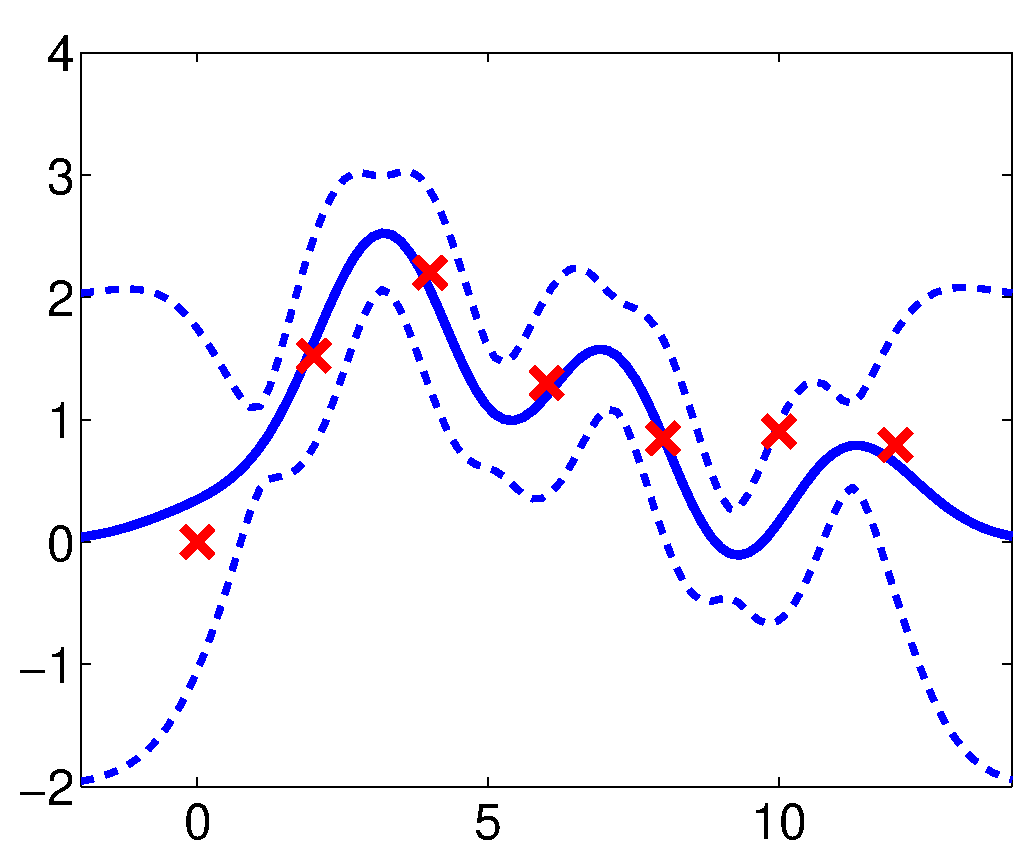
\includegraphics[%
  width=0.45\textwidth]{../diagrams/demBarenco1_profile1_slides}}\subfigure[]{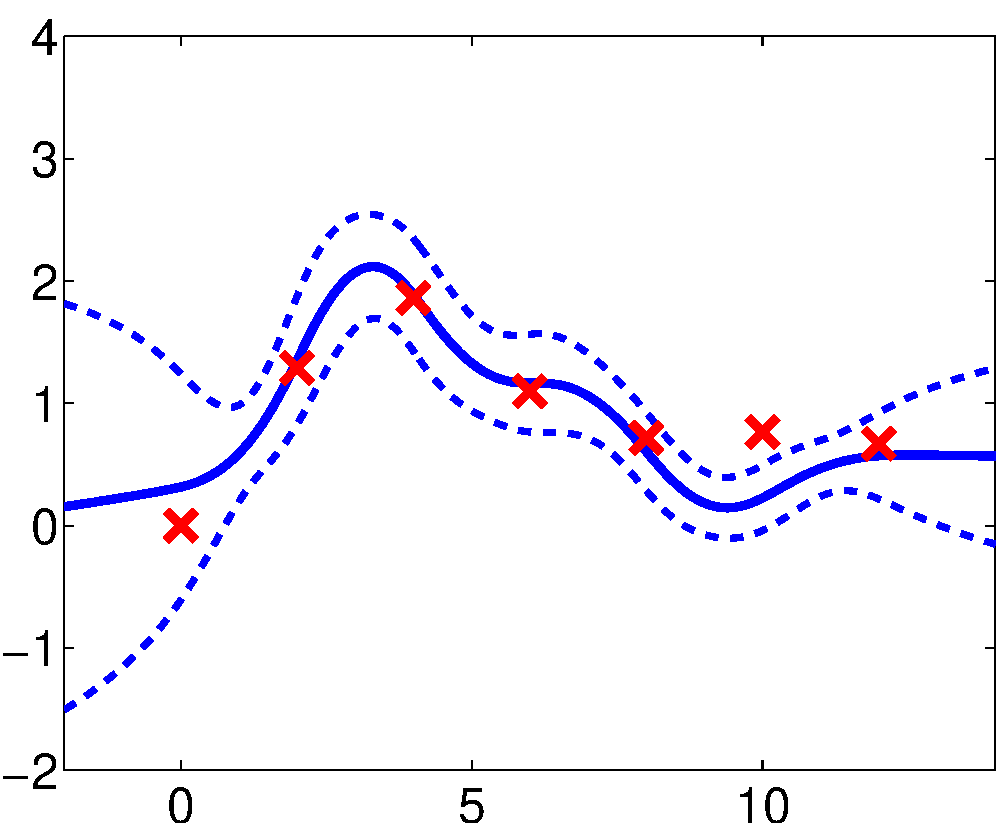
\includegraphics[%
  width=0.45\textwidth]{../diagrams/demBarencoMap2MlpLinear_profile1_slide}}
\end{center}
\vspace{-0.4cm}

\caption{\small Predicted protein concentration for p53 using a linear response 
model: (a) squared exponential prior on $f$; (b) MLP prior on $f$. Solid line is mean 
prediction, dashed
lines are 95\% credibility intervals. 
The prediction of Barenco \emph{et al.} was pointwise and is shown as crosses.}
\label{cap:barencoComparisonProfile}\vspace{-0.3cm}
\end{figure}%
\begin{figure}[ht]\vspace{-0.2cm}
\begin{center}\subfigure[]{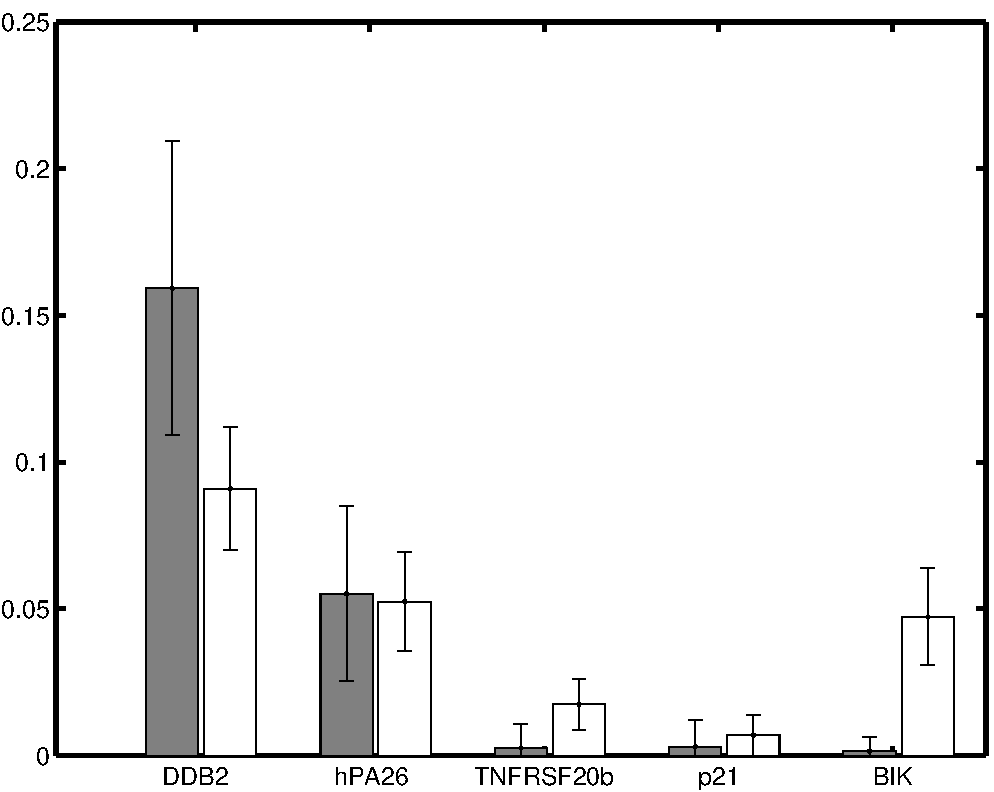
\includegraphics[%
  width=0.30\textwidth]{../diagrams/HMCBaseErrBars}}\hfill{}\subfigure[]{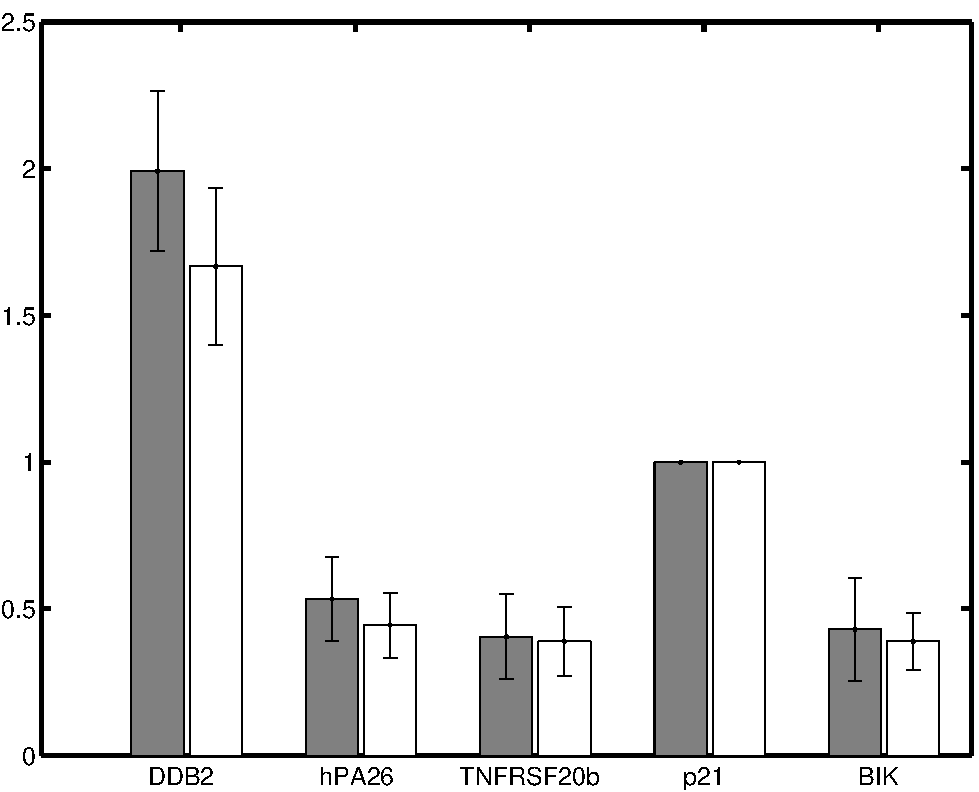
\includegraphics[%
  width=0.30\textwidth]{../diagrams/HMCSensErrBars}}\hfill{}\subfigure[]{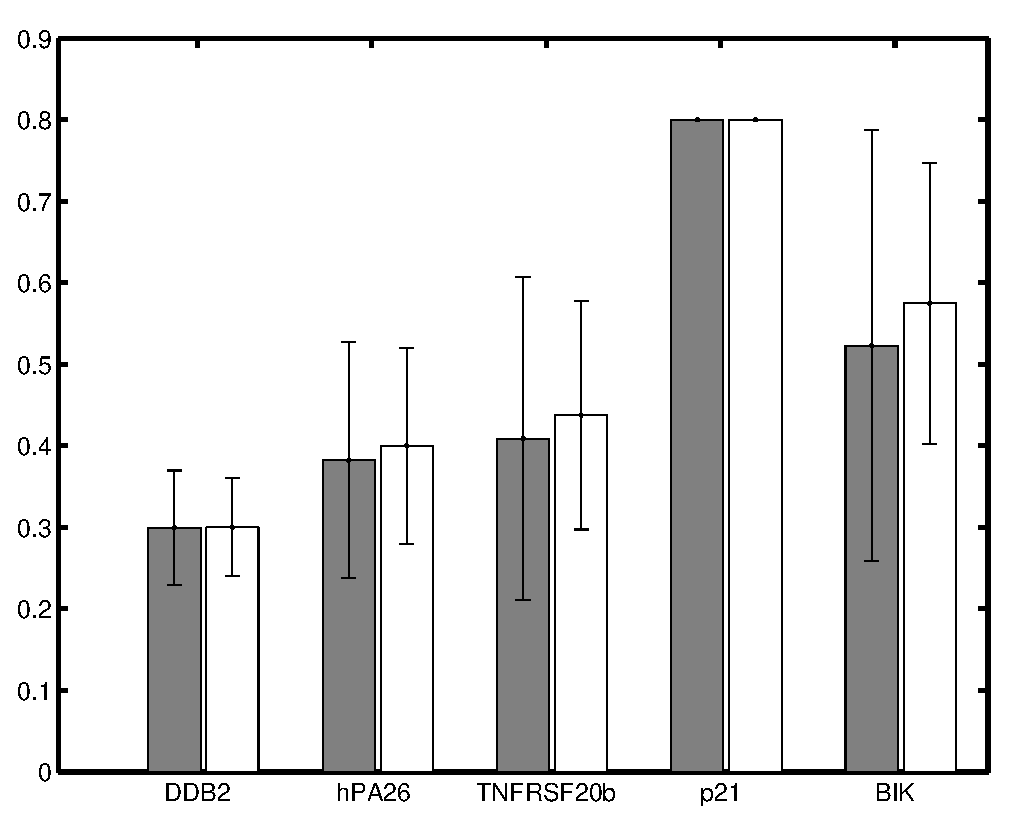
\includegraphics[%
  width=0.30\textwidth]{../diagrams/HMCDecayErrBars}}\end{center}

\vspace{-0.8cm}
\caption{\small Results of inference on the hyperparameters for p53 data studied in \cite{Barenco:ranked06}.
The bar charts show (a) Basal transcription rates from our model and
that of Barenco \emph{et al.}. Grey are estimates obtained with our model, 
white are the estimates obtained by Barenco \emph{et al.} 
(b) Similar for sensitivities.
(c) Similar for decay rates.\label{cap:barencoComparisonBar}}\vspace{-0.3cm}
\end{figure}

Figure~\ref{cap:barencoComparisonBar} shows the results of inference on the 
values of the hyperparameters $B_j$, $S_j$ and $D_j$. The columns on the left,
shaded grey, show results from our model and the white columns are the
estimates obtained in \cite{Barenco:ranked06}. The hyperparameters were assigned a 
vague gamma prior distribution ($a=b=0.1$, corresponding to a mean of 1 and a 
variance of 10). Samples from the posterior distribution were obtained using
Hybrid Monte Carlo \cite[see \emph{e.g.}][]{Neal:book96}. The results are
in good accordance with the results obtained by Barenco \emph{et al.} 
Differences in the estimates of the basal transcription rates are probably 
due to the different methods used for probe-level processing of the microarray
data. 
\subsection{Non-linear response analysis}
We then used the non-linear response model of section \ref{sec:nonlinear} in 
order to constrain the protein concentrations inferred to be positive. We 
achieved this by using an exponential response of the transcription rate to 
the logged protein concentration. 
The inferred MAP solutions for the latent function $f$ are plotted in Figure
\ref{nonlinearInf} for the squared exponential prior (a) and for the MLP prior
(b).

%
\begin{figure}[ht]\vspace{-0.4cm}
\begin{center}\subfigure[]{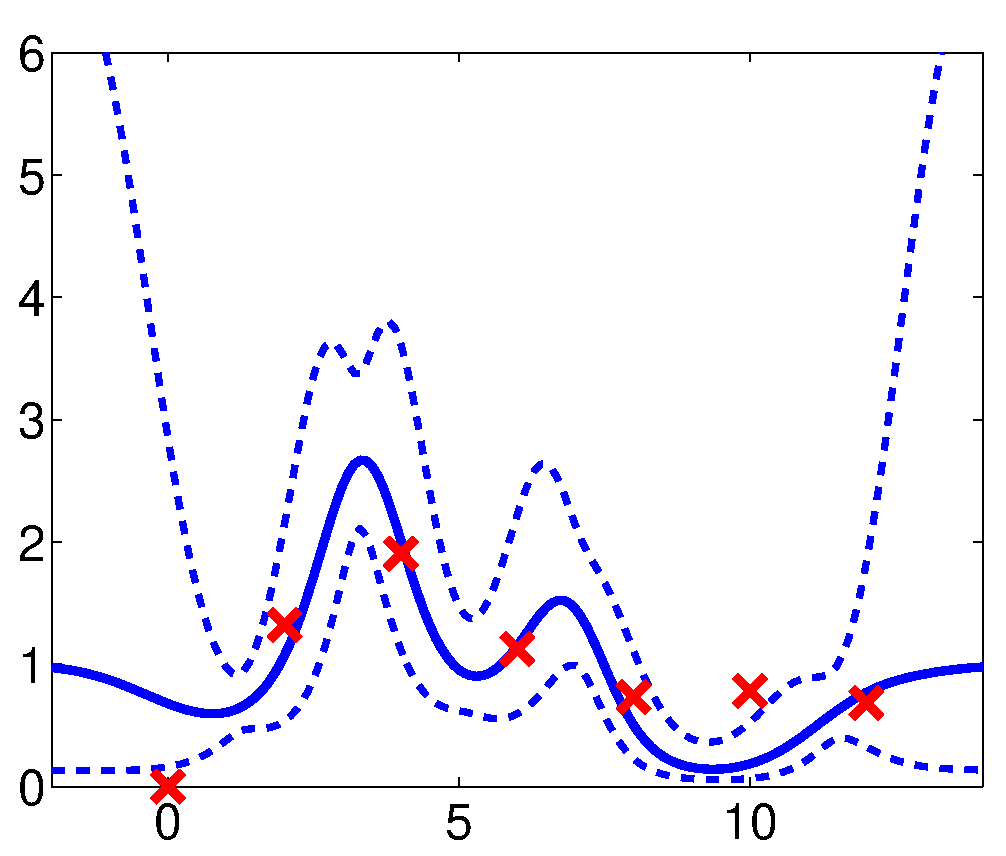
\includegraphics[%
  width=0.45\textwidth]{../diagrams/demBarencoMap3RbfExp_profile1_slide}}\subfigure[]{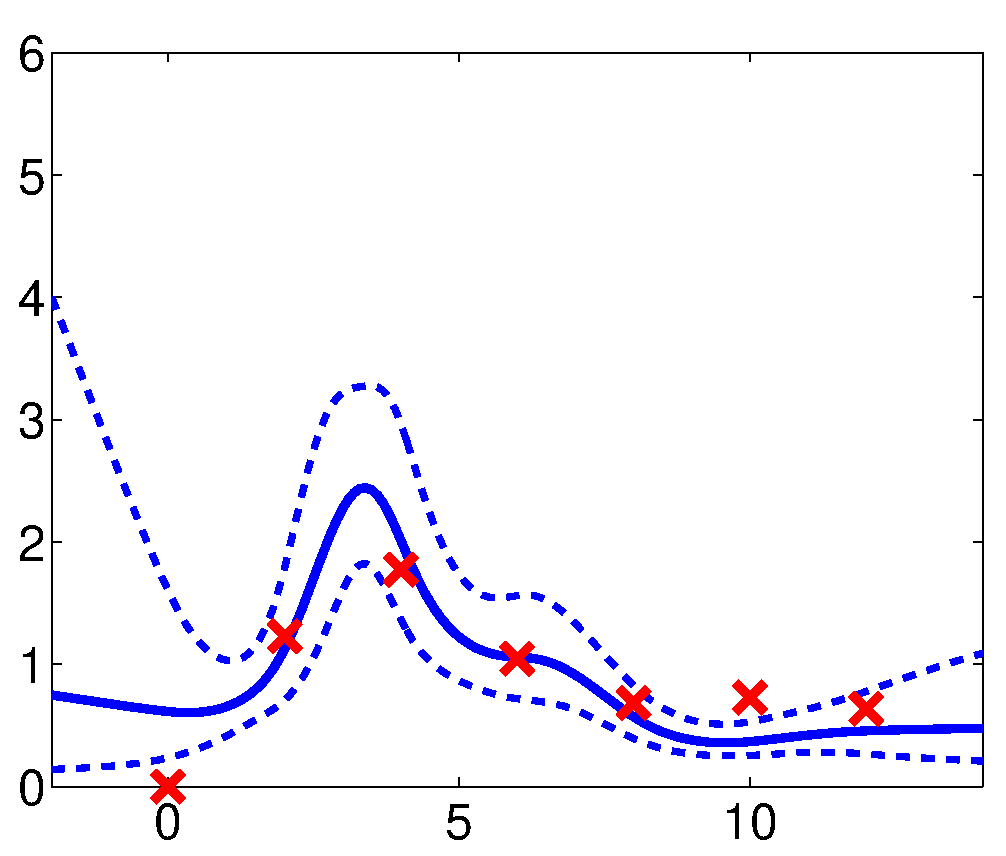
\includegraphics[%
  width=0.45\textwidth]{../diagrams/demBarencoMap4MlpExp_profile1_slide}}
\end{center}\vspace{-0.4cm}
\caption{\small Predicted protein concentration for p53 using an exponential response:
(a) shows results of using a squared exponential prior covariance on $f$; (b) 
shows results of using an MLP prior covariance on $f$.
Solid line is mean 
prediction, dashed
lines show 95\% credibility intervals. The results shown are for 
$\textrm{exp}(f)$, hence the asymmetry of the credibility intervals. 
The prediction of Barenco \emph{et al.} was pointwise and is shown as crosses.}
\label{nonlinearInf}\vspace{-0.3cm}
\end{figure}%
\section{Discussion}
In this paper we showed how Gaussian processes can be used effectively
in modelling the dynamics of a very simple regulatory network motif.
This approach has many advantages over standard parametric approaches:
first of all, there is no need to restrict the inference to the
observed time points, and the temporal continuity of the inferred
functions is accounted for naturally. Secondly, Gaussian processes
allow noise information to be accounted for in a natural way. It is
well known that biological data exhibits a large variability, partly
because of technical noise (due to the difficulty to measure mRNA
abundance for low expressed genes, for example), and partly because of
the difference between different cell lines. Accounting for these
sources of noise in a parametric model can be difficult (particularly
when estimates of the derivatives of the measured quantities are
required), while Gaussian Processes can incorporate this information
naturally. Finally, MCMC parameter estimation in a discretised model
can be computationally expensive due to the high correlations between
variables. This is a consequence of treating the protein
concentrations as parameters, and results in many MCMC iterations to
obtain reliable samples.  Parameter estimation can be achieved easily
in our framework by type II maximum likelihood or by using efficient
Monte Carlo sampling techniques only on the model hyperparameters.

While the results shown in the paper are encouraging, this is still a very 
simple modelling situation. For example, it is well known that transcriptional 
delays can play a significant role in determining the dynamics of many
cellular processes \cite{Monk03}. These effects can be introduced naturally
in a Gaussian process model; however, the data must be sampled at a reasonably
high frequency in order for delays to become identifiable in a stochastic 
model, which is often not the case with microarray data sets. Another natural
extension of our work would be to consider more biologically meaningful
nonlinearities, such as the popular Michaelis-Menten model of transcription 
used in \cite{Rogers:model06b}. Finally, networks consisting of a single
transcription factor are very useful
to study small systems of particular interest such as p53. However, our 
ultimate goal would be to describe regulatory pathways consisting of
more genes. These can be
dealt with in the general framework described in this paper, but 
careful thought
will be needed to overcome the greater computational difficulties.

\subsection*{Acknowledgements}

We thank Martino Barenco for useful discussions and for
providing the data. We gratefully acknowledge support from BBSRC Grant No BBS/B/0076X ``Improved processing of microarray data with probabilistic models''.
%\bibliographystyle{plainnat}
\small
\bibliographystyle{abbrv}
\bibliography{gpip}



\end{document}